\documentclass{beamer}
\usetheme{Madrid}
\usecolortheme{whale}
\usepackage{tikz}
\usetikzlibrary{positioning}
\usepackage{booktabs}
\setbeamertemplate{navigation symbols}{}
\setbeamertemplate{footline}[frame number]

\title{Risk Management Fundamentals}
\author{Presenter Name}
\date{\today}

\begin{document}

\begin{frame}
\titlepage
\end{frame}

\begin{frame}
\frametitle{Introduction: Understanding Risk Management Fundamentals}
\begin{itemize}
  \item \textbf{Risk management} is the systematic process of identifying, assessing, and controlling threats to an organization's operations and objectives.
  \item Effective risk management allows organizations to prepare for the unexpected and minimize both the likelihood and impact of negative events.
  \item Risk management is a continuous process that evolves as the organization and its environment change over time.
  \item All stakeholders have a role to play in the risk management process, from frontline employees to executive leadership.
\end{itemize}

\begin{alertblock}{Why Risk Management Matters}
Without structured risk management, organizations face unexpected disruptions, financial losses, reputation damage, and potential regulatory consequences.
\end{alertblock}
\end{frame}

\begin{frame}
\frametitle{The Risk Management Process: An Overview}
\begin{itemize}
  \item The risk management process follows a structured approach to handling potential threats and opportunities.
  \item Effective risk management begins with comprehensive \textbf{risk identification} to discover what could affect your objectives.
  \item \textbf{Risk assessment and analysis} help you understand the significance and potential impact of identified risks.
  \item After analyzing risks, organizations implement \textbf{risk response strategies} to address each risk appropriately.
\end{itemize}

\begin{center}
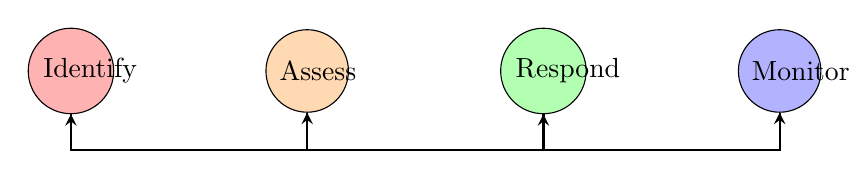
\begin{tikzpicture}
% Define styles for nodes and edges
\tikzstyle{identify} = [circle, draw, fill=red!30, text width=2em, text centered, minimum height=2em]
\tikzstyle{assess} = [circle, draw, fill=orange!30, text width=2em, text centered, minimum height=2em]
\tikzstyle{respond} = [circle, draw, fill=green!30, text width=2em, text centered, minimum height=2em]
\tikzstyle{monitor} = [circle, draw, fill=blue!30, text width=2em, text centered, minimum height=2em]
\tikzstyle{arrow} = [thick,->,>=stealth]

% Nodes
\node[identify] (identify) {Identify};
\node[assess, right of=identify, node distance=3cm] (assess) {Assess};
\node[respond, right of=assess, node distance=3cm] (respond) {Respond};
\node[monitor, right of=respond, node distance=3cm] (monitor) {Monitor};

% Edges
\draw[arrow] (identify) -- ++(0,-1) -| (assess);
\draw[arrow] (assess) -- ++(0,-1) -| (respond);
\draw[arrow] (respond) -- ++(0,-1) -| (monitor);
\draw[arrow] (monitor) -- ++(0,-1) -| (identify);
\end{tikzpicture}
\end{center}
\end{frame}

\begin{frame}
\frametitle{Risk Identification: Finding Potential Threats}
\begin{itemize}
  \item \textbf{Risk identification} is the process of determining what could happen that might affect objectives and how those things might happen.
  \item Effective risk identification considers both internal factors (processes, systems, people) and external factors (economic, political, technological).
  \item Risk identification should be comprehensive, capturing both obvious and less apparent risks that could impact the organization.
  \item The output of risk identification becomes the input to the next stages of the risk management process.
\end{itemize}

\begin{block}{Common Sources of Risk}
\begin{itemize}
  \item Strategic risks: Competition, industry changes, customer demand
  \item Operational risks: Systems failures, supply chain issues, human errors
  \item Financial risks: Market fluctuations, credit issues, liquidity problems
  \item Compliance risks: Regulatory changes, legal requirements, standards
\end{itemize}
\end{block}
\end{frame}

\begin{frame}
    \frametitle{Tools and Techniques for Effective Risk Identification}
    \begin{itemize}
      \item \textbf{Brainstorming sessions} bring together diverse perspectives to identify potential risks that might not be obvious to individuals.
      \item \textbf{Checklists and questionnaires} provide structured approaches to ensure common risks aren't overlooked in the identification process.
      \item \textbf{Historical data analysis} examines past incidents and near-misses to identify patterns and potential future risks.
      \item \textbf{SWOT analysis} (Strengths, Weaknesses, Opportunities, Threats) helps identify risks in the context of the organization's overall position.
    \end{itemize}
    
    \begin{table}
    \centering
    \begin{tabular}{ll}
    \toprule
    \textbf{Technique} & \textbf{Best Used For} \\
    \midrule
    Brainstorming & Unique or complex projects \\
    Checklists & Routine operations \\
    Historical Analysis & Recurring processes \\
    Expert Interviews & Specialized or technical areas \\
    \bottomrule
    \end{tabular}
    \end{table}
    \end{frame}
    
    \begin{frame}
    \frametitle{Introduction to Risk Assessment}
    \begin{itemize}
      \item \textbf{Risk assessment} is the process of evaluating identified risks to determine their significance to the organization.
      \item Assessment helps organizations prioritize which risks require immediate attention and which can be addressed later.
      \item Effective risk assessment considers both the likelihood of a risk occurring and the potential impact if it does occur.
      \item Risk assessment can be performed using different approaches depending on the nature of the risks and organizational needs.
    \end{itemize}
    
    \begin{block}{The Risk Assessment Process}
    Assessment transforms a list of identified risks into actionable information by determining which risks matter most and require immediate response strategies.
    \end{block}
    \end{frame}
    
    \begin{frame}
    \frametitle{Ad Hoc Risk Assessment: When and How to Use It}
    \begin{itemize}
      \item \textbf{Ad hoc risk assessment} is conducted on an as-needed basis in response to specific events or changes in the environment.
      \item This approach is useful when unexpected situations arise that weren't covered in regular assessment processes.
      \item Ad hoc assessments are typically focused on a specific issue rather than comprehensively evaluating all organizational risks.
      \item While informal in nature, ad hoc assessments should still follow structured methodology to ensure quality results.
    \end{itemize}
    
    \begin{exampleblock}{Example: Ad Hoc Assessment Trigger}
    When a competitor launches a surprise new product that threatens market share, an ad hoc assessment might be initiated to evaluate the competitive risk and develop immediate response strategies.
    \end{exampleblock}
    \end{frame}
    
\begin{frame}
\frametitle{Recurring Risk Assessments: Building Systematic Approaches}
\begin{itemize}
  \item \textbf{Recurring risk assessments} are performed at regular intervals (monthly, quarterly, annually) as part of normal operations.
  \item This systematic approach ensures that risk profiles are regularly updated to reflect changing conditions.
  \item Recurring assessments often follow standardized procedures, making them efficient and consistent over time.
  \item The frequency of recurring assessments should match the pace of change in the risk environment and organizational needs.
\end{itemize}
\begin{center}
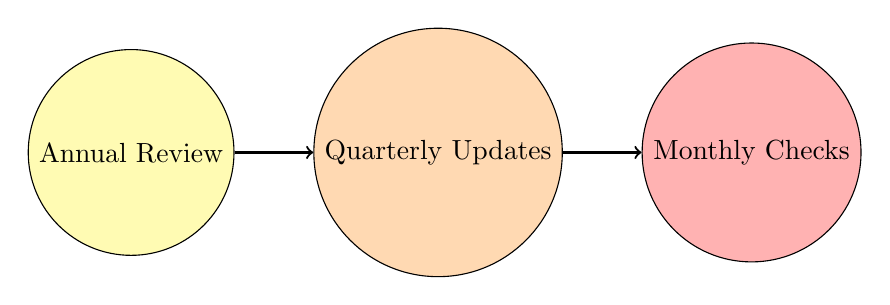
\begin{tikzpicture}
% Nodes
\node[circle, draw, fill=yellow!30, minimum size=1.5cm] (annual) {Annual Review};
\node[circle, draw, fill=orange!30, minimum size=1.2 cm, right=1cm of annual] (quarterly) {Quarterly Updates};
\node[circle, draw, fill=red!30, minimum size=1cm, right=1cm of quarterly] (monthly) {Monthly Checks};

% Edges
\draw[->, thick] (annual) -- (quarterly);
\draw[->, thick] (quarterly) -- (monthly);
\end{tikzpicture}
\end{center}
\end{frame}


\begin{frame}
  \frametitle{One-Time Risk Assessments: Special Projects and Events}
  \begin{itemize}
    \item \textbf{One-time risk assessments} are conducted for specific projects, events, or decisions that are not part of routine operations.
    \item These assessments are tailored to the unique characteristics of the situation and typically have a defined endpoint.
    \item One-time assessments are essential when launching new products, entering new markets, or making significant organizational changes.
    \item The scope of a one-time assessment should be clearly defined to ensure all relevant risks are captured without becoming unwieldy.
  \end{itemize}
  
  \begin{block}{When to Use One-Time Assessments}
  \begin{itemize}
    \item Major capital investments
    \item Mergers and acquisitions
    \item New product launches
    \item Facility relocations
  \end{itemize}
  \end{block}
  \end{frame}
  
  \begin{frame}
  \frametitle{Continuous Risk Assessment: Creating an Ongoing Culture of Awareness}
  \begin{itemize}
    \item \textbf{Continuous risk assessment} involves constantly monitoring the environment for emerging risks and changing conditions.
    \item This approach integrates risk awareness into daily operations rather than treating it as a separate activity.
    \item Continuous assessment relies on real-time data and feedback mechanisms to provide early warning of potential issues.
    \item Organizations with mature risk management programs often evolve toward continuous assessment approaches.
  \end{itemize}
  
  \begin{alertblock}{Benefit of Continuous Assessment}
  Continuous assessment allows organizations to identify and respond to risks more quickly than traditional periodic assessments, potentially preventing small issues from becoming major problems.
  \end{alertblock}
  \end{frame}
  
  \begin{frame}
  \frametitle{Risk Analysis: Moving from Identification to Understanding}
  \begin{itemize}
    \item \textbf{Risk analysis} involves examining identified risks to determine their characteristics, causes, and potential consequences.
    \item Effective analysis provides the foundation for making informed decisions about how to respond to each risk.
    \item Risk analysis can range from simple, intuitive approaches to complex mathematical models depending on the situation.
    \item The depth of analysis should be proportional to the potential impact of the risk and the resources available.
  \end{itemize}
  
  \begin{block}{Types of Risk Analysis}
  There are three main types of risk analysis:
  \scriptsize
  \begin{itemize}
    \item \textbf{Qualitative Analysis}: Uses descriptive categories (e.g., high, medium, low) to assess the likelihood and impact of risks based on expert judgment and experience.
    \item \textbf{Semi-Quantitative Analysis}: Combines elements of both qualitative and quantitative analysis, often using numerical scales to rate risks while still relying on expert judgment.
    \item \textbf{Quantitative Analysis}: Uses numerical data and statistical methods to calculate the probability and impact of risks, providing a more precise and objective assessment.
  \end{itemize}
  \end{block}
  \end{frame}
  
  \begin{frame}
  \frametitle{Qualitative Risk Analysis: Using Expert Judgment}
  \begin{itemize}
    \item \textbf{Qualitative risk analysis} uses descriptive scales (high/medium/low) rather than numerical values to assess risks.
    \item This approach relies heavily on expert judgment, experience, and stakeholder input to evaluate risks.
    \item Qualitative analysis is useful when numerical data is limited or when a quick assessment is needed.
    \item The results of qualitative analysis are typically presented in risk matrices that map likelihood against impact.
  \end{itemize}
  
  \begin{table}
  \centering
  \begin{tabular}{l|ccc}
  \textbf{Impact} & \multicolumn{3}{c}{\textbf{Likelihood}} \\
   & Low & Medium & High \\
  \hline
  High & Medium & High & High \\
  Medium & Low & Medium & High \\
  Low & Low & Low & Medium \\
  \end{tabular}
  \caption{Simple Qualitative Risk Matrix}
  \end{table}
  \end{frame}
  
  \begin{frame}
    \frametitle{Quantitative Risk Analysis: Putting Numbers to Risk}
    \begin{itemize}
      \item \textbf{Quantitative risk analysis} uses numerical values and statistical techniques to evaluate risks with precision.
      \item This approach assigns specific values to the probability of occurrence and the potential financial impact of risks.
      \item Quantitative analysis provides more objective measurements than qualitative methods but requires more data and resources.
      \item The results of quantitative analysis help prioritize risks based on their expected monetary value.
    \end{itemize}
    
    \begin{exampleblock}{Quantitative Analysis Formula}
    \begin{center}
    Risk Exposure = Probability of Risk Occurrence × Impact of Risk
    \end{center}
    \end{exampleblock}
    \end{frame}
    
    \begin{frame}
    \frametitle{Single Loss Expectancy (SLE): Calculating Individual Risk Events}
    \begin{itemize}
      \item \textbf{Single Loss Expectancy (SLE)} represents the monetary value expected to be lost from a single occurrence of a risk event.
      \item SLE is calculated by multiplying the asset value by the exposure factor (percentage of asset lost in the event).
      \item This metric helps organizations understand the potential impact of individual risk events when they occur.
      \item SLE is a building block for more comprehensive risk calculations like Annualized Loss Expectancy.
    \end{itemize}
    
    \begin{block}{SLE Formula}
    \begin{center}
    SLE = Asset Value × Exposure Factor
    \end{center}
    \textbf{Example:} If a server worth \$100,000 would be 25\% damaged by a power surge, the SLE would be \$25,000.
    \end{block}
    \end{frame}
    
    \begin{frame}
    \frametitle{Annualized Loss Expectancy (ALE): Projecting Yearly Impact}
    \begin{itemize}
      \item \textbf{Annualized Loss Expectancy (ALE)} estimates the expected monetary loss from a specific risk over a one-year period.
      \item ALE is calculated by multiplying the Single Loss Expectancy (SLE) by the Annualized Rate of Occurrence (ARO).
      \item This metric allows organizations to compare different risks on an annual basis for budgeting and prioritization.
      \item ALE provides a common financial language for discussing risk with executives and other stakeholders.
    \end{itemize}
    
    \begin{table}
    \centering
    \begin{tabular}{lrrrr}
    \toprule
    \textbf{Risk Event} & \textbf{Asset Value} & \textbf{EF} & \textbf{ARO} & \textbf{ALE} \\
    \midrule
    Power Outage & \$100,000 & 10\% & 2 & \$20,000 \\
    Data Breach & \$500,000 & 40\% & 0.1 & \$20,000 \\
    Hardware Failure & \$50,000 & 100\% & 0.5 & \$25,000 \\
    \bottomrule
    \end{tabular}
    \end{table}
    \end{frame}
    
    \begin{frame}
    \frametitle{Annualized Rate of Occurrence (ARO): Understanding Risk Frequency}
    \begin{itemize}
      \item \textbf{Annualized Rate of Occurrence (ARO)} represents how often a specific risk event is expected to happen in a year.
      \item ARO can be a whole number (such as 12 for monthly events) or a fraction (such as 0.1 for events expected once per decade).
      \item ARO is typically estimated using historical data, industry statistics, and expert judgment.
      \item Understanding frequency is crucial for determining which risks require immediate mitigation versus long-term planning.
    \end{itemize}
    
    \begin{center}
    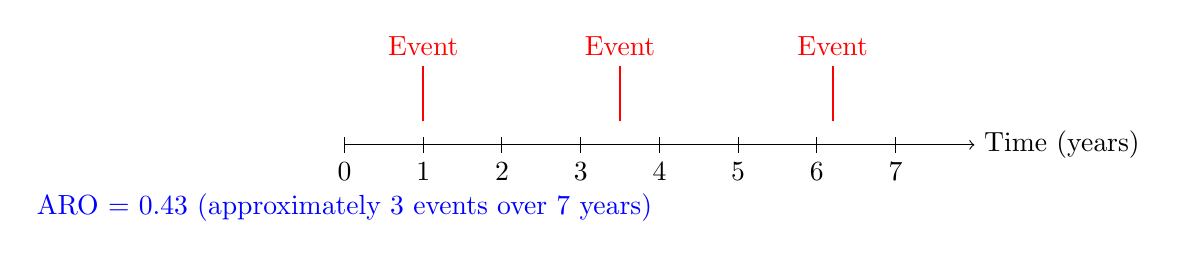
\begin{tikzpicture}
    \draw[->] (0,0) -- (8,0) node[right] {Time (years)};
    \foreach \x in {0,1,2,3,4,5,6,7}
        \draw (\x,0.1) -- (\x,-0.1) node[below] {\x};
    \draw[red,thick] (1,0.3) -- (1,1) node[above] {Event};
    \draw[red,thick] (3.5,0.3) -- (3.5,1) node[above] {Event};
    \draw[red,thick] (6.2,0.3) -- (6.2,1) node[above] {Event};
    \draw[blue] (0,-0.5) node[below] {ARO = 0.43 (approximately 3 events over 7 years)};
    \end{tikzpicture}
    \end{center}
    \end{frame}


    \begin{frame}
      \frametitle{Probability, Likelihood and Exposure: Key Risk Measurements}
      \begin{itemize}
        \item \textbf{Probability} refers to the mathematical chance that a risk event will occur, often expressed as a percentage.
        \item \textbf{Likelihood} is a more qualitative assessment of how likely an event is to happen (e.g., rare, unlikely, possible, likely, almost certain).
        \item \textbf{Exposure factor (EF)} is the percentage of an asset that would be lost if a specific risk event occurs.
        \item These measurements work together to provide a complete picture of risk potential and severity.
      \end{itemize}
      
      \begin{table}
      \centering
      \begin{tabular}{ll}
      \toprule
      \textbf{Likelihood Category} & \textbf{Approximate Probability} \\
      \midrule
      Rare & $<1\%$ chance per year \\
      Unlikely & $1-10\%$ chance per year \\
      Possible & $10-50\%$ chance per year \\
      Likely & $50-90\%$ chance per year \\
      Almost Certain & $>90\%$ chance per year \\
      \bottomrule
      \end{tabular}
      \end{table}
      \end{frame}
      
      \begin{frame}
      \frametitle{Impact Assessment: Understanding Consequences of Risk Events}
      \begin{itemize}
        \item \textbf{Impact} refers to the severity of consequences if a risk event occurs, often measured across multiple dimensions.
        \item Comprehensive impact assessment considers financial, operational, reputational, and strategic effects of risk events.
        \item Impact scales can be qualitative (minor, moderate, major) or quantitative (specific dollar amounts or percentages).
        \item Organizations should develop impact criteria that reflect their unique priorities and risk context.
      \end{itemize}
      
      \begin{block}{Multi-dimensional Impact Assessment}
      \begin{itemize}
        \item \textbf{Financial:} Direct monetary losses, costs, fines
        \item \textbf{Operational:} Disruption to business activities
        \item \textbf{Reputational:} Damage to brand and stakeholder trust
        \item \textbf{Strategic:} Effect on long-term objectives
        \item \textbf{Compliance:} Regulatory consequences
      \end{itemize}
      \end{block}
      \end{frame}
      
      \begin{frame}
      \frametitle{The Risk Register: Documenting Your Risk Landscape}
      \begin{itemize}
        \item The \textbf{risk register} is a centralized document that records identified risks along with their analysis and planned responses.
        \item An effective risk register serves as both a communication tool and a management record throughout the risk process.
        \item Risk registers should be living documents that are regularly reviewed and updated as conditions change.
        \item The level of detail in a risk register should match the complexity of the organization and the risks being managed.
      \end{itemize}
      
      \begin{exampleblock}{Key Elements of a Risk Register}
      \begin{itemize}
        \item Risk ID and description
        \item Risk category and source
        \item Probability and impact assessments
        \item Current controls and their effectiveness
        \item Response strategies and action plans
        \item Risk owner and status updates
      \end{itemize}
      \end{exampleblock}
      \end{frame}
      
      \begin{frame}
      \frametitle{Key Risk Indicators: Early Warning Signs}
      \begin{itemize}
        \item \textbf{Key Risk Indicators (KRIs)} are metrics that provide early warning signals about increasing risk exposure.
        \item Effective KRIs are predictive, measurable, and linked to specific risks that matter to the organization.
        \item KRIs should have defined thresholds that trigger specific actions when crossed, creating a proactive response system.
        \item Regular monitoring of KRIs helps organizations detect emerging risks before they materialize into significant problems.
      \end{itemize}
      
      \begin{center}
      \begin{tikzpicture}
      \draw[->] (0,0) -- (8,0) node[right] {Time};
      \draw[->] (0,0) -- (0,4) node[above] {Risk Level};
      
      % Draw threshold lines
      \draw[dashed, red] (0,3) -- (8,3) node[right] {Threshold};
      
      % Draw the metric line
      \draw[thick, blue] (0,1) -- (2,1.2) -- (3,1.4) -- (4,2) -- (5,2.5) -- (6,3.2) -- (7,3.5) -- (8,3.8);
      
      % Mark the threshold crossing
      \draw[thick, red, ->] (5.9,3.5) -- (5.9,3.1) node[below right] {Action Required};
      
      \end{tikzpicture}
      \end{center}
      \end{frame}

      \begin{frame}
        \frametitle{Risk Owners: Assigning Accountability}
        \begin{itemize}
          \item \textbf{Risk owners} are individuals responsible for managing specific risks, including monitoring, response planning, and reporting.
          \item Effective risk ownership requires clear delegation of authority and responsibility to someone with appropriate skills and resources.
          \item Risk owners are accountable for keeping risk information current and implementing approved response strategies.
          \item Without clear ownership, risks often fall through organizational cracks and remain unaddressed.
        \end{itemize}
        
        \begin{block}{Responsibilities of Risk Owners}
        The risk owner is responsible for understanding the risk, developing response plans, implementing controls, monitoring effectiveness, and reporting status to stakeholders regularly.
        \end{block}
        \end{frame}
        
        \begin{frame}
        \frametitle{Risk Thresholds: Knowing When to Act}
        \begin{itemize}
          \item \textbf{Risk thresholds} are predetermined levels at which a risk becomes unacceptable and requires specific actions.
          \item Thresholds are often linked to key risk indicators and provide objective criteria for escalation and response.
          \item Well-designed thresholds help organizations respond consistently to changing risk levels across different areas.
          \item Thresholds should be set through a collaborative process involving risk owners, management, and other stakeholders.
        \end{itemize}
        
        \begin{center}
        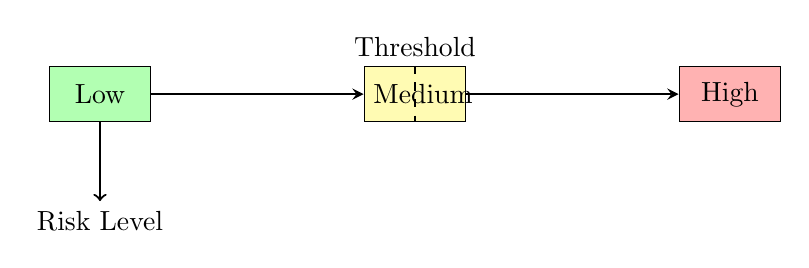
\begin{tikzpicture}
        % Define styles for nodes and edges
        \tikzstyle{low} = [rectangle, draw, fill=green!30, text width=3em, text centered, minimum height=2em]
        \tikzstyle{medium} = [rectangle, draw, fill=yellow!30, text width=3em, text centered, minimum height=2em]
        \tikzstyle{high} = [rectangle, draw, fill=red!30, text width=3em, text centered, minimum height=2em]
        \tikzstyle{arrow} = [thick,->,>=stealth]

        % Nodes
        \node[low] (low) {Low};
        \node[medium, right of=low, node distance=4cm] (medium) {Medium};
        \node[high, right of=medium, node distance=4cm] (high) {High};

        % Arrows
        \draw[arrow] (low) -- (medium);
        \draw[arrow] (medium) -- (high);

        % Threshold line
        \draw[dashed, thick] (medium.north) -- (medium.south);
        \node[above] at (medium.north) {Threshold};

        % Risk level indicator
        \draw[thick, ->] (low.south) -- ++(0,-1) node[below] {Risk Level};
        \end{tikzpicture}
        \end{center}
        \end{frame}
        \begin{frame}
        \frametitle{Risk Tolerance: How Much Risk Can You Handle?}
        \begin{itemize}
          \item \textbf{Risk tolerance} refers to an organization's ability to withstand a specific amount of risk before experiencing significant harm.
          \item Tolerance levels vary across different risk categories and are influenced by organizational resources and resilience.
          \item Understanding tolerance helps organizations determine which risks require immediate action versus those that can be accepted.
          \item Risk tolerance should be explicitly defined and communicated to ensure consistent decision-making throughout the organization.
        \end{itemize}
        
        \begin{exampleblock}{Examples of Risk Tolerance Statements}
        \begin{itemize}
          \item Financial: "We can tolerate up to \$500,000 in unexpected losses without affecting our strategic objectives."
          \item Operational: "We can accept up to 4 hours of system downtime per quarter with minimal business impact."
          \item Reputational: "We have zero tolerance for ethics violations that could damage our brand reputation."
        \end{itemize}
        \end{exampleblock}
        \end{frame}
        
        \begin{frame}
        \frametitle{Risk Appetite: Strategic Approaches to Risk}
        \begin{itemize}
          \item \textbf{Risk appetite} is the amount and type of risk an organization is willing to take in pursuit of its strategic objectives.
          \item Unlike tolerance (ability to withstand risk), appetite reflects a deliberate choice about how much risk to pursue.
          \item Risk appetite is typically set by senior leadership and the board as part of the strategic planning process.
          \item A well-defined risk appetite guides decision-making and resource allocation throughout the organization.
        \end{itemize}
        
        \begin{alertblock}{Risk Appetite vs. Risk Tolerance}
        Risk appetite is a strategic choice about how much risk to pursue, while risk tolerance is the operational ability to withstand risk. An organization might have a high appetite for strategic growth risks but low tolerance for compliance risks.
        \end{alertblock}
        \end{frame}

        \begin{frame}
          \frametitle{Expansionary, Conservative, and Neutral Risk Profiles}
          \begin{itemize}
            \item An \textbf{expansionary risk profile} reflects a high appetite for risk in pursuit of growth, innovation, and market leadership.
            \item A \textbf{conservative risk profile} prioritizes stability and protection of existing assets over potentially risky growth opportunities.
            \item A \textbf{neutral risk profile} balances risk-taking and risk-aversion, seeking moderate growth while maintaining reasonable protection.
            \item Most organizations adopt different risk profiles for different aspects of their operations rather than a single approach.
          \end{itemize}
          
          \begin{table}
          \centering
          \begin{tabular}{lccc}
          \toprule
          \textbf{Characteristics} & \textbf{Expansionary} & \textbf{Neutral} & \textbf{Conservative} \\
          \midrule
          Growth Focus & High & Moderate & Low \\
          Innovation & Aggressive & Selective & Cautious \\
          New Markets & Early Entry & Follower & Late Entry \\
          Investment Strategy & Higher Risk & Balanced & Lower Risk \\
          \bottomrule
          \end{tabular}
          \end{table}
          \end{frame}
          
          \begin{frame}
          \frametitle{Risk Management Strategies: Making Decisions}
          \begin{itemize}
            \item \textbf{Risk management strategies} are the approaches used to address identified and assessed risks.
            \item The selection of an appropriate strategy depends on the nature of the risk, its severity, and the organization's risk appetite.
            \item Most organizations employ a mix of strategies across their risk portfolio rather than a single approach.
            \item The choice of strategy should consider both the costs and benefits of implementation relative to the risk exposure.
          \end{itemize}
          
          \begin{exampleblock}{Common Risk Management Strategies}
            \scriptsize
          \begin{itemize}
            \item \textbf{Risk Avoidance:} Taking actions to eliminate the risk entirely, such as discontinuing a risky activity.
            \item \textbf{Risk Mitigation:} Implementing measures to reduce the likelihood or impact of the risk, such as installing security systems.
            \item \textbf{Risk Transfer:} Shifting the risk to another party, typically through insurance or outsourcing.
            \item \textbf{Risk Acceptance:} Acknowledging the risk and deciding to retain it without specific actions, often because the cost of mitigation is higher than the potential impact.
          \end{itemize}
          \end{exampleblock}
          \end{frame}
          
          \begin{frame}
          \frametitle{Risk Transfer: Sharing the Burden}
          \begin{itemize}
            \item \textbf{Risk transfer} involves shifting the responsibility for managing a risk to another party, typically through insurance or contracts.
            \item This strategy is appropriate when the organization lacks the expertise or resources to manage the risk effectively.
            \item Common transfer mechanisms include insurance policies, service agreements, and partnerships with specialized providers.
            \item While risk transfer can reduce exposure, organizations must be aware that some aspects of risk (especially reputational) cannot be fully transferred.
          \end{itemize}
          
          \begin{exampleblock}{Examples of Risk Transfer}
          \begin{itemize}
            \item Purchasing property insurance to transfer financial impact of facility damage
            \item Using a cloud service provider to transfer some IT infrastructure risks
            \item Hiring specialized contractors for hazardous activities
            \item Entering into fixed-price contracts to transfer cost escalation risks
          \end{itemize}
          \end{exampleblock}
          \end{frame}
          
          \begin{frame}
          \frametitle{Risk Acceptance: When to Live with Risk}
          \begin{itemize}
            \item \textbf{Risk acceptance} involves acknowledging a risk and deciding to retain it without taking specific action to address it.
            \item Acceptance is appropriate when the cost of other risk responses exceeds the potential benefit or when the risk is within tolerance levels.
            \item \textbf{Exemptions} are formal decisions to accept risks that exceed normal thresholds due to special circumstances.
            \item \textbf{Exceptions} are temporary approvals to operate outside normal risk parameters for a specified period.
          \end{itemize}
          
          \begin{alertblock}{Important Note on Risk Acceptance}
          Risk acceptance is not the same as ignoring risk. Proper acceptance requires formal acknowledgment, documentation, and ongoing monitoring of the accepted risk to ensure it remains within tolerable levels.
          \end{alertblock}
          \end{frame}

          \begin{frame}
            \frametitle{Risk Avoidance: Eliminating Threats}
            \begin{itemize}
              \item \textbf{Risk avoidance} involves making decisions that completely eliminate specific risk exposures.
              \item This strategy typically means not engaging in certain activities, exiting markets, or discontinuing products that carry unacceptable risks.
              \item Avoidance is appropriate when a risk presents significant threats with limited opportunities for effective control.
              \item While avoidance eliminates specific risks, it may also eliminate potential rewards or create other risks that must be considered.
            \end{itemize}
            
            \begin{block}{Examples of Risk Avoidance}
            \begin{itemize}
              \item Deciding not to expand into a politically unstable region
              \item Discontinuing a product line with significant liability concerns
              \item Rejecting a project with environmental compliance challenges
              \item Divesting from a business unit facing overwhelming regulatory pressure
            \end{itemize}
            \end{block}
            \end{frame}
            
            \begin{frame}
            \frametitle{Risk Mitigation: Reducing Impact and Likelihood}
            \begin{itemize}
              \item \textbf{Risk mitigation} involves taking actions to reduce either the likelihood of a risk occurring or the impact if it does occur.
              \item Mitigation is the most common risk response strategy and covers a wide range of actions tailored to specific risks.
              \item Effective mitigation often involves multiple layers of controls to provide defense in depth against potential threats.
              \item The cost and effectiveness of mitigation measures should be proportional to the level of risk being addressed.
            \end{itemize}
            
            \begin{center}
            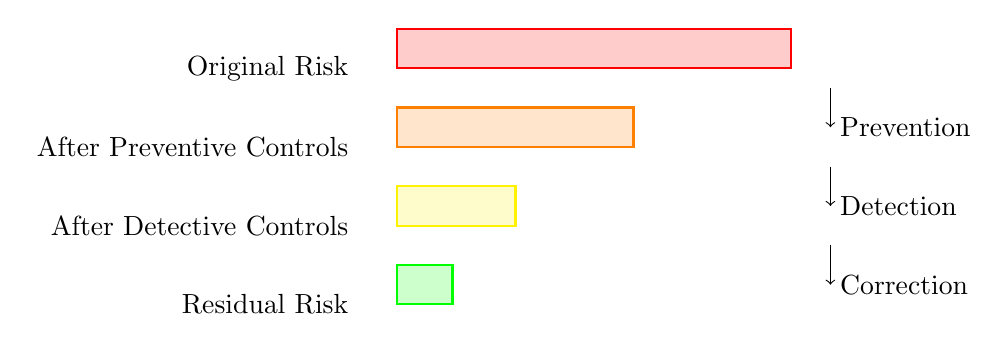
\begin{tikzpicture}
            \draw (0,0) node[anchor=east] {Original Risk};
            \draw (0,-1) node[anchor=east] {After Preventive Controls};
            \draw (0,-2) node[anchor=east] {After Detective Controls};
            \draw (0,-3) node[anchor=east] {Residual Risk};
            
            \draw[thick, red, fill=red!20] (0.5,0) rectangle +(5,0.5);
            \draw[thick, orange, fill=orange!20] (0.5,-1) rectangle +(3,0.5);
            \draw[thick, yellow, fill=yellow!20] (0.5,-2) rectangle +(1.5,0.5);
            \draw[thick, green, fill=green!20] (0.5,-3) rectangle +(0.7,0.5);
            
            \draw[->] (6,-0.25) -- (6,-0.75) node[right] {Prevention};
            \draw[->] (6,-1.25) -- (6,-1.75) node[right] {Detection};
            \draw[->] (6,-2.25) -- (6,-2.75) node[right] {Correction};
            \end{tikzpicture}
            \end{center}
            \end{frame}
            
            \begin{frame}
            \frametitle{Risk Reporting: Communicating to Stakeholders}
            \begin{itemize}
              \item \textbf{Risk reporting} involves communicating relevant risk information to internal and external stakeholders in a timely manner.
              \item Effective reporting provides transparency about the organization's risk profile, controls, and management activities.
              \item Reports should be tailored to the needs of different audiences, from operational teams to executive leadership to external regulators.
              \item Regular reporting builds accountability and ensures that risk management remains a priority throughout the organization.
            \end{itemize}
            
            \begin{table}
            \centering
            \begin{tabular}{lll}
            \toprule
            \textbf{Audience} & \textbf{Reporting Focus} & \textbf{Frequency} \\
            \midrule
            Board & Strategic risks, risk appetite & Quarterly \\
            Executive Team & Key risk indicators, emerging risks & Monthly \\
            Risk Committee & Control effectiveness, risk trends & Monthly \\
            Operational Managers & Specific risk areas, action items & Weekly \\
            \bottomrule
            \end{tabular}
            \end{table}
            \end{frame}
            
            \begin{frame}
            \frametitle{Business Impact Analysis: Planning for Disruption}
            \begin{itemize}
              \item \textbf{Business Impact Analysis (BIA)} is the process of determining the effect of disruptions on critical business functions.
              \item \textbf{Recovery Time Objective (RTO)} defines the maximum acceptable time to restore a process after a disruption.
              \item \textbf{Recovery Point Objective (RPO)} defines the maximum acceptable data loss measured in time.
              \item \textbf{Mean Time to Repair (MTTR)} and \textbf{Mean Time Between Failures (MTBF)} help quantify system reliability and recovery capabilities.
            \end{itemize}
            
            \begin{exampleblock}{BIA Process Overview}
            \begin{enumerate}
              \item Identify critical business functions and processes
              \item Determine impacts of disruption over time
              \item Establish recovery priorities and timeframes
              \item Identify resource requirements for recovery
              \item Document findings and recommendations
            \end{enumerate}
            \end{exampleblock}
            \end{frame}

            \begin{frame}
              \frametitle{Conclusion: Building a Comprehensive Risk Management Program}
              \scriptsize
              \begin{itemize}
                \item Effective risk management requires a holistic approach that integrates all elements of the risk process into organizational operations.
                \item A mature risk management program evolves from reactive to proactive, continuously improving based on experience and changing conditions.
                \item Risk management is everyone's responsibility, though different roles have different accountabilities within the program.
                \item When properly implemented, risk management becomes a strategic advantage rather than just a compliance exercise.
              \end{itemize}
              
              \begin{center}
              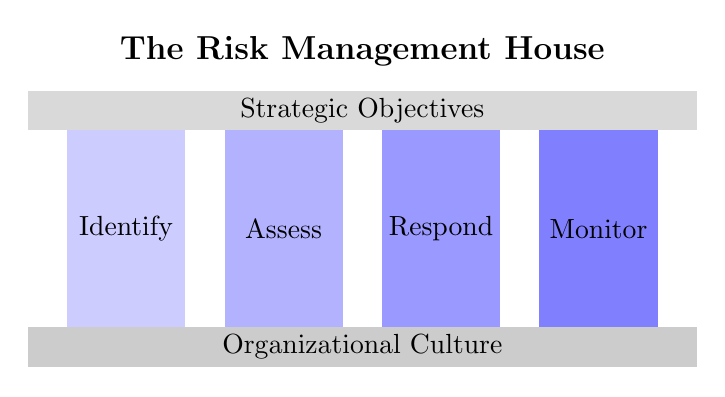
\begin{tikzpicture}
              % Create pillars of risk management
              \fill[blue!20] (0,0) rectangle (1.5,2.5);
              \node[text width=1.5cm, align=center] at (0.75,1.25) {Identify};
              
              \fill[blue!30] (2,0) rectangle (3.5,2.5);
              \node[text width=1.5cm, align=center] at (2.75,1.25) {Assess};
              
              \fill[blue!40] (4,0) rectangle (5.5,2.5);
              \node[text width=1.5cm, align=center] at (4.75,1.25) {Respond};
              
              \fill[blue!50] (6,0) rectangle (7.5,2.5);
              \node[text width=1.5cm, align=center] at (6.75,1.25) {Monitor};
              
              % Add foundation and roof
              \fill[gray!40] (-0.5,-0.5) rectangle (8,0);
              \node at (3.75,-0.25) {Organizational Culture};
              
              \fill[gray!30] (-0.5,2.5) rectangle (8,3);
              \node at (3.75,2.75) {Strategic Objectives};
              
              % Add title
              \node at (3.75,3.5) {\large \textbf{The Risk Management House}};
              \end{tikzpicture}
              \end{center}
              \end{frame}
        
\end{document}